\subsubsection{Paklaida ir tikslumas}

Abiejų metodų paklaidos ir tikslumo kreivės palygintos~\ref{fig:bgd_vs_sgd_error} ir~\ref{fig:bgd_vs_sgd_accuracy} paveiksluose.

\begin{figure}[H]
    \centering
    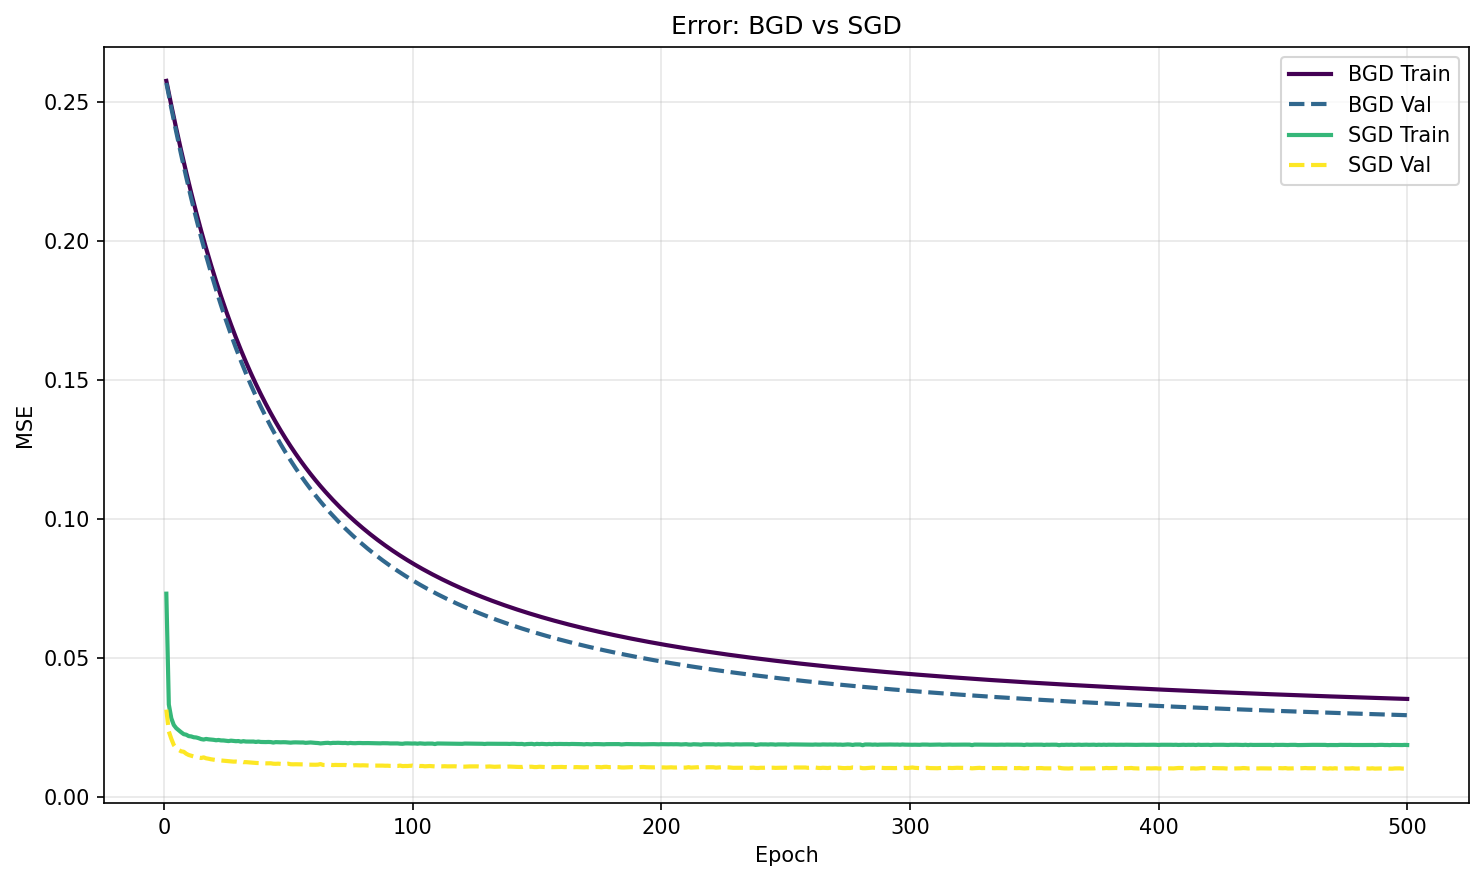
\includegraphics[width=0.85\linewidth]{2Lab/visualizations/bgd_vs_sgd_error.png}
    \caption{Paklaidos palyginimas: paketinis ir stochastinis GN}
    \label{fig:bgd_vs_sgd_error}
\end{figure}

\begin{figure}[H]
    \centering
    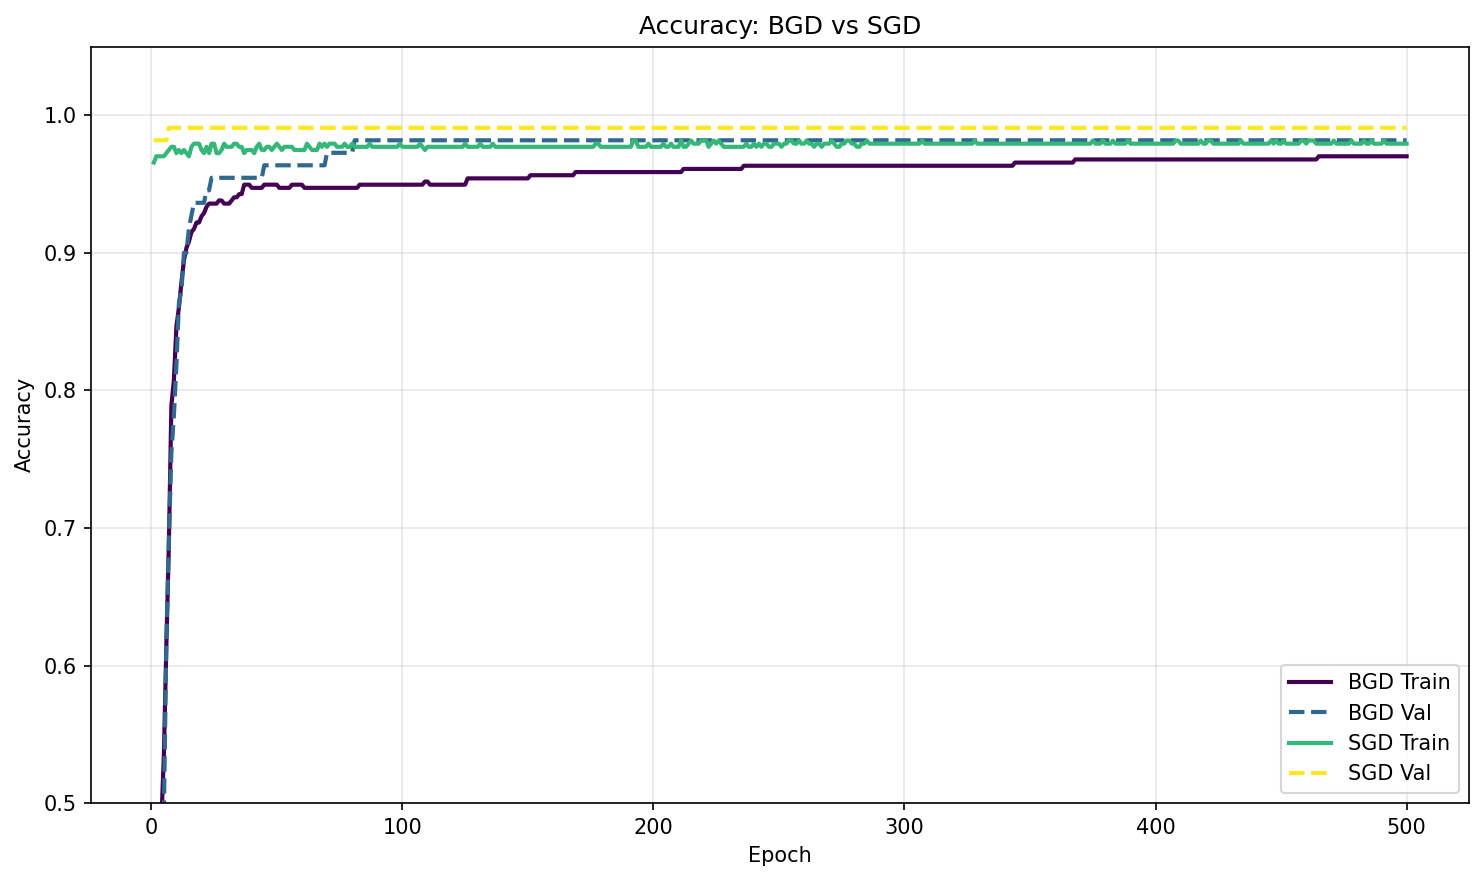
\includegraphics[width=0.85\linewidth]{2Lab/visualizations/bgd_vs_sgd_accuracy.png}
    \caption{Tikslumo palyginimas: paketinis ir stochastinis GN}
    \label{fig:bgd_vs_sgd_accuracy}
\end{figure}

Stochastinis gradientinis nusileidimas pasiekia mažesnę paklaidą ir aukštesnį validavimo tikslumą ($99{,}1\ \%$) nei paketinis ($98{,}2\ \%$). Tačiau testavimo duomenims paketinis metodas pasiekia aukštesnį tikslumą ($97{,}1\ \%$) nei stochastinis ($95{,}6\ \%$), o tai rodo, kad stochastinis metodas gali šiek tiek persimokyti validavimo duomenims (žr.~\ref{fig:bgd_vs_sgd_val_accuracy} pav.).

\begin{figure}[H]
    \centering
    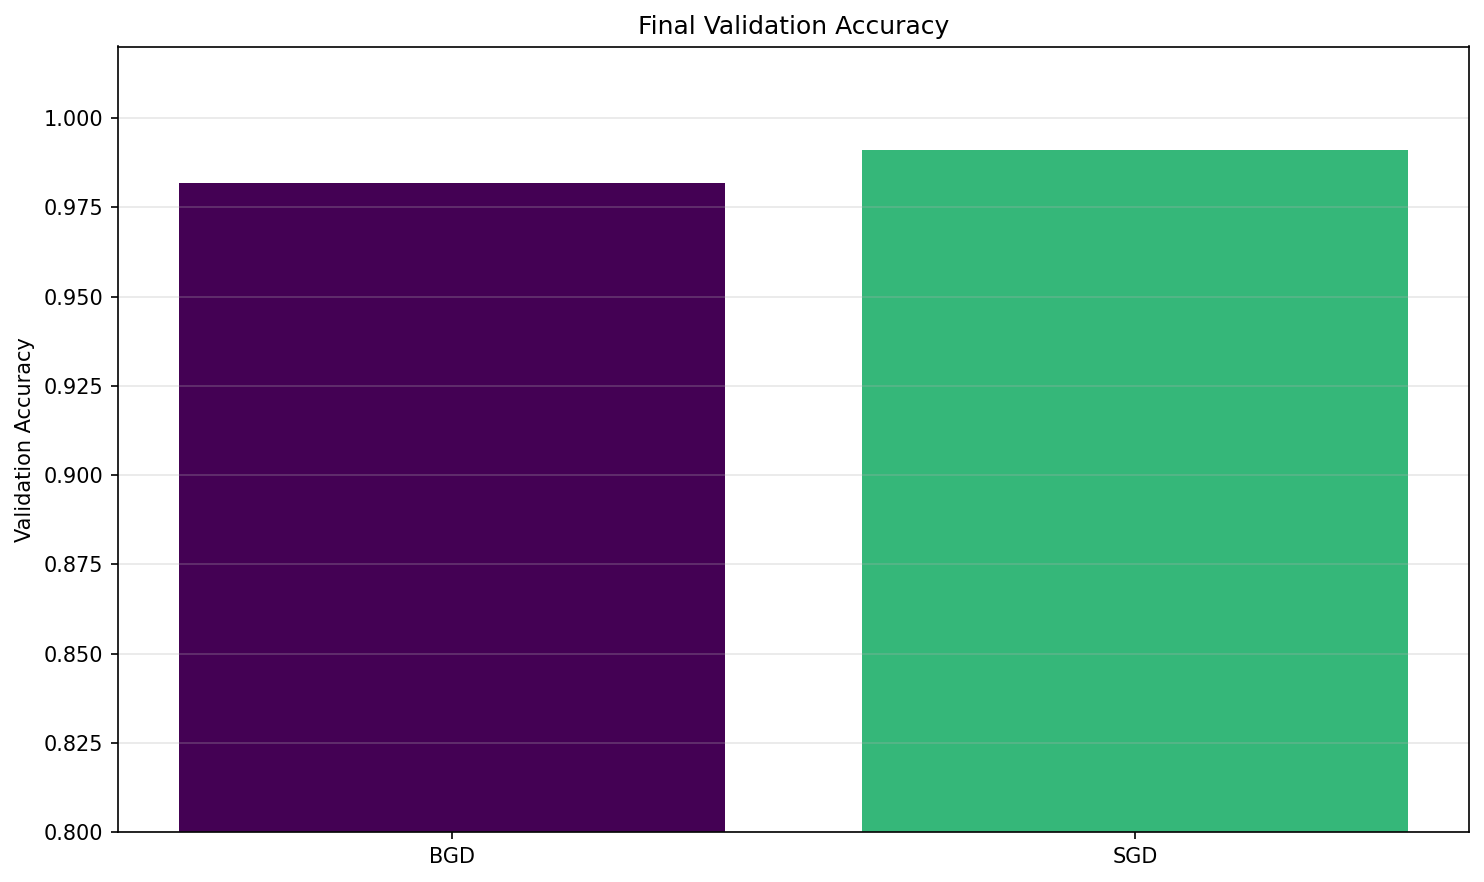
\includegraphics[width=0.85\linewidth]{2Lab/visualizations/bgd_vs_sgd_val_accuracy.png}
    \caption{Galutinis validavimo tikslumas: paketinis ir stochastinis GN}
    \label{fig:bgd_vs_sgd_val_accuracy}
\end{figure}